\section{Applications}

AI is being employed to good effect in areas including:

\begin{itemize}
    \item Pattern Recognition (e.g.: face/image recognition)
    \item Classification (e.g.: fault diagnosis, DNA analysis)
    \item Associative Memory (e.g.: image compression)
    \item Clustering (e.g.: credit analysis, fraud prevention)
\end{itemize}
with additional applications in Aerospace, Finance, Medical, Security, Transport, etc \cite{Garcez2019}.  

Areas of particular interest due to high profile results include Natural Language Processing (NLP) and Computer Vision. Other areas that are increasingly making use of AI include DSP, as an example LSTM-based approaches to classifying transient radio frequency interference \cite{Czech2018}. This could be employed for products subject to EMC testing.  

\begin{figure}[ht]
 \centering % avoid the use of \begin{center}...\end{center} and use \centering instead (more compact)
 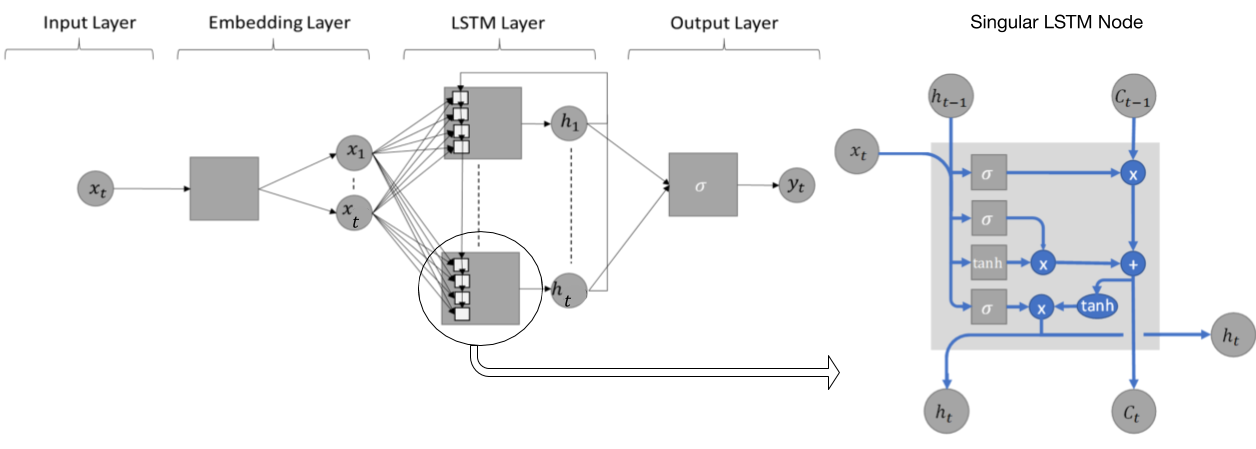
\includegraphics[width=160mm]{images/LSTM.png}
 \caption{Long Short-Term Memory (LSTM) Network diagram generated by Matlab desktop application}
 \label{fig:sample}
\end{figure}

Although Deep Networks have brought the promise of generating classifiers that do away for the need of domain knowledge, but in reality domain knowledge is still pivotal in designing and adjusting neural networks and is also necessary in collecting and processing data, which will become training, validation and testing datasets for candidate classifier models. It is generally agreed that it is important to start small \cite{ELMAN199371}, and also to normalize data, to deal with complex industrial problems \cite{589532}.  
